\begin{tikzpicture}
  %% \begin{tikzpicture}[gnuplot]
%% generated with GNUPLOT 4.6p0 (Lua 5.1; terminal rev. 99, script rev. 100)
%% Tue 04 Dec 2012 03:00:09 PM CST
\path (0.000,0.000) rectangle (12.500,8.750);
\gpcolor{color=gp lt color border}
\gpsetlinetype{gp lt border}
\gpsetlinewidth{1.00}
\draw[gp path] (1.504,0.985)--(1.684,0.985);
\draw[gp path] (11.947,0.985)--(11.767,0.985);
\node[gp node right] at (1.320,0.985) { 0};
\draw[gp path] (1.504,2.464)--(1.684,2.464);
\draw[gp path] (11.947,2.464)--(11.767,2.464);
\node[gp node right] at (1.320,2.464) { 0.2};
\draw[gp path] (1.504,3.943)--(1.684,3.943);
\draw[gp path] (11.947,3.943)--(11.767,3.943);
\node[gp node right] at (1.320,3.943) { 0.4};
\draw[gp path] (1.504,5.423)--(1.684,5.423);
\draw[gp path] (11.947,5.423)--(11.767,5.423);
\node[gp node right] at (1.320,5.423) { 0.6};
\draw[gp path] (1.504,6.902)--(1.684,6.902);
\draw[gp path] (11.947,6.902)--(11.767,6.902);
\node[gp node right] at (1.320,6.902) { 0.8};
\draw[gp path] (1.504,8.381)--(1.684,8.381);
\draw[gp path] (11.947,8.381)--(11.767,8.381);
\node[gp node right] at (1.320,8.381) { 1};
\draw[gp path] (1.504,0.985)--(1.504,1.165);
\draw[gp path] (1.504,8.381)--(1.504,8.201);
\node[gp node center] at (1.504,0.677) { 0};
\draw[gp path] (2.639,0.985)--(2.639,1.165);
\draw[gp path] (2.639,8.381)--(2.639,8.201);
\node[gp node center] at (2.639,0.677) { 5};
\draw[gp path] (3.774,0.985)--(3.774,1.165);
\draw[gp path] (3.774,8.381)--(3.774,8.201);
\node[gp node center] at (3.774,0.677) { 10};
\draw[gp path] (4.909,0.985)--(4.909,1.165);
\draw[gp path] (4.909,8.381)--(4.909,8.201);
\node[gp node center] at (4.909,0.677) { 15};
\draw[gp path] (6.044,0.985)--(6.044,1.165);
\draw[gp path] (6.044,8.381)--(6.044,8.201);
\node[gp node center] at (6.044,0.677) { 20};
\draw[gp path] (7.180,0.985)--(7.180,1.165);
\draw[gp path] (7.180,8.381)--(7.180,8.201);
\node[gp node center] at (7.180,0.677) { 25};
\draw[gp path] (8.315,0.985)--(8.315,1.165);
\draw[gp path] (8.315,8.381)--(8.315,8.201);
\node[gp node center] at (8.315,0.677) { 30};
\draw[gp path] (9.450,0.985)--(9.450,1.165);
\draw[gp path] (9.450,8.381)--(9.450,8.201);
\node[gp node center] at (9.450,0.677) { 35};
\draw[gp path] (10.585,0.985)--(10.585,1.165);
\draw[gp path] (10.585,8.381)--(10.585,8.201);
\node[gp node center] at (10.585,0.677) { 40};
\draw[gp path] (11.720,0.985)--(11.720,1.165);
\draw[gp path] (11.720,8.381)--(11.720,8.201);
\node[gp node center] at (11.720,0.677) { 45};
\draw[gp path] (1.504,8.381)--(1.504,0.985)--(11.947,0.985)--(11.947,8.381)--cycle;
\node[gp node center,rotate=-270] at (0.246,4.683) {Electrons per pulse (a.u.)};
\node[gp node center] at (6.725,0.215) {Laser Intensity (MW/cm$^2$)};
\gpcolor{color=gp lt color 0}
\gpsetlinetype{gp lt plot 0}
\gpsetlinewidth{2.00}
\draw[gp path] (11.904,8.381)--(11.896,8.352)--(11.833,8.187)--(11.745,7.731)--(11.632,7.885)%
  --(11.496,7.798)--(11.336,7.673)--(11.154,7.602)--(10.950,7.393)--(10.725,7.463)--(10.482,7.261)%
  --(10.219,7.186)--(9.940,4.874)--(9.645,3.229)--(9.336,2.517)--(9.014,2.034)--(8.682,1.795)%
  --(8.339,1.731)--(7.989,1.699)--(7.632,1.610)--(7.271,1.461)--(6.908,1.394)--(6.543,1.430)%
  --(6.180,1.345)--(5.819,1.273)--(5.462,1.235)--(5.112,1.178)--(4.769,1.147)--(4.437,1.119)%
  --(4.115,1.103)--(3.806,1.082)--(3.511,1.072)--(3.232,1.038)--(2.969,1.009);
\gpcolor{color=gp lt color 1}
\gpsetlinetype{gp lt plot 1}
\draw[gp path] (3.311,0.985)--(3.511,0.997)--(3.806,0.995)--(4.115,1.000)--(4.437,1.000)%
  --(4.769,1.011)--(5.112,1.014)--(5.462,1.026)--(5.819,1.036)--(6.180,1.043)--(6.543,1.045)%
  --(6.908,1.071)--(7.271,1.092)--(7.632,1.106)--(7.989,1.119)--(8.339,1.146)--(8.682,1.168)%
  --(9.014,1.176)--(9.336,1.195)--(9.645,1.238)--(9.940,1.248)--(10.219,1.267)--(10.482,1.258)%
  --(10.725,1.301)--(10.950,1.312)--(11.154,1.338)--(11.336,1.351)--(11.496,1.354)--(11.632,1.375)%
  --(11.745,1.393)--(11.833,1.400)--(11.896,1.382)--(11.934,1.415)--(11.947,1.398);
\gpcolor{color=gp lt color border}
\gpsetlinetype{gp lt border}
\gpsetlinewidth{1.00}
\draw[gp path] (1.504,8.381)--(1.504,0.985)--(11.947,0.985)--(11.947,8.381)--cycle;
%% coordinates of the plot area
\gpdefrectangularnode{gp plot 1}{\pgfpoint{1.504cm}{0.985cm}}{\pgfpoint{11.947cm}{8.381cm}}
%% \end{tikzpicture}
%% gnuplot variables


  \node at (0,-1.5) {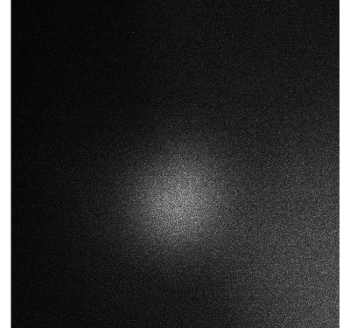
\includegraphics{final-fourier-022.png}};
  \node [white] at (-1, -0.5) {A};
  \draw [thick,->] (6.5,3) -- ++(0,-1.5) node [pos=0,above] {A};

  \node at (3,-1.5) {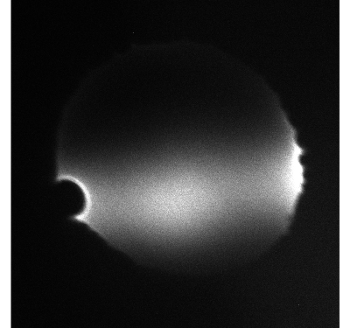
\includegraphics{final-fourier-026.png}};
  \node [white] at (2, -0.5) {B};
  \draw [thick,->] (8,3) -- ++(0,-1.2) node [pos=0,above] {B};

  \node at (6,-1.5) {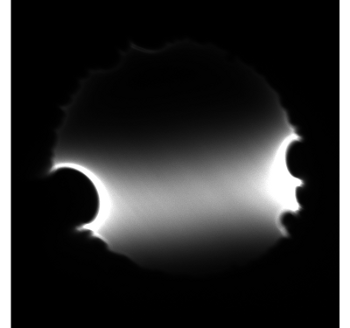
\includegraphics{final-fourier-030.png}};
  \node [white] at (5, -0.5) {C};
  \draw [thick,->] (9,4) -- ++(-80:1.3) node [pos=0,above] {C};

  \node at (9,-1.5) {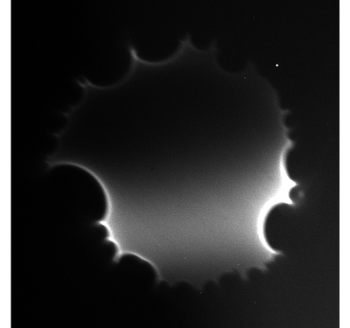
\includegraphics{final-fourier-038.png}};
  \node [white] at (8, -0.5) {D};
  \draw [thick,<-] (11.3,7.5) -- ++(0,-1.5) node [pos=1,below] {D};

  \node at (12,-1.5) {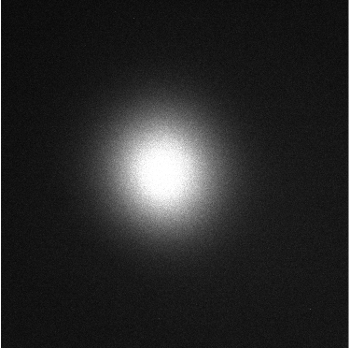
\includegraphics{final-fourier-2photon-036.png}};
  \node [white] at (11, -0.5) {E};
  \draw [thick,->] (11,3) -- ++(0,-1.5) node [pos=0,above] {E};
\end{tikzpicture}
